% This file was created by matlab2tikz.
%
\definecolor{mycolor1}{rgb}{0.06600,0.44300,0.74500}%
\definecolor{mycolor2}{rgb}{0.12941,0.12941,0.12941}%
\definecolor{mycolor3}{rgb}{0.86600,0.32900,0.00000}%
\definecolor{mycolor4}{rgb}{0.92900,0.69400,0.12500}%
\definecolor{mycolor5}{rgb}{0.52100,0.08600,0.81900}%
\definecolor{mycolor6}{rgb}{0.23100,0.66600,0.19600}%
\definecolor{mycolor7}{rgb}{0.18400,0.74500,0.93700}%
\definecolor{mycolor8}{rgb}{0.81900,0.01500,0.54500}%
%
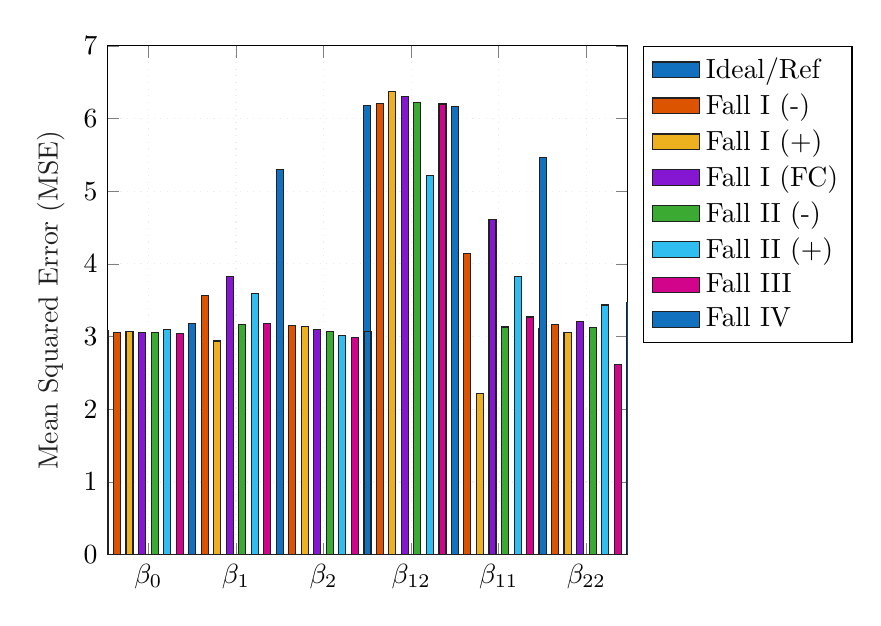
\begin{tikzpicture}

\begin{axis}[%
width=0.545\textwidth,
height=0.533\textwidth,
at={(0\textwidth,0\textwidth)},
scale only axis,
bar shift auto,
xmin=0.5300,
xmax=6.4700,
xtick={1.0000,2.0000,3.0000,4.0000,5.0000,6.0000},
xticklabels={{$\beta_0$},{$\beta_1$},{$\beta_2$},{$\beta_{12}$},{$\beta_{11}$},{$\beta_{22}$}},
ymin=0.0000,
ymax=7.0000,
ylabel style={font=\color{mycolor2}},
ylabel={Mean Squared Error (MSE)},
axis background/.style={fill=white},
xmajorgrids,
ymajorgrids,
grid style={dotted, opacity=0.25},
legend style={at={(1.03,1)}, anchor=north west, legend cell align=left, align=left}
]
\addplot[ybar, bar width=0.08, fill=mycolor1, draw=mycolor2, area legend] table[row sep=crcr] {%
1.0000	3.0894\\
2.0000	3.0976\\
3.0000	3.1664\\
4.0000	6.1732\\
5.0000	3.1269\\
6.0000	3.1053\\
};
\addplot[forget plot, color=mycolor2] table[row sep=crcr] {%
0.5300	0.0000\\
6.4700	0.0000\\
};
\addlegendentry{Ideal/Ref}

\addplot[ybar, bar width=0.08, fill=mycolor3, draw=mycolor2, area legend] table[row sep=crcr] {%
1.0000	3.0519\\
2.0000	3.5687\\
3.0000	3.1473\\
4.0000	6.2035\\
5.0000	4.1459\\
6.0000	3.1668\\
};
\addplot[forget plot, color=mycolor2] table[row sep=crcr] {%
0.5300	0.0000\\
6.4700	0.0000\\
};
\addlegendentry{Fall I (-)}

\addplot[ybar, bar width=0.08, fill=mycolor4, draw=mycolor2, area legend] table[row sep=crcr] {%
1.0000	3.0668\\
2.0000	2.9390\\
3.0000	3.1412\\
4.0000	6.3668\\
5.0000	2.2138\\
6.0000	3.0597\\
};
\addplot[forget plot, color=mycolor2] table[row sep=crcr] {%
0.5300	0.0000\\
6.4700	0.0000\\
};
\addlegendentry{Fall I (+)}

\addplot[ybar, bar width=0.08, fill=mycolor5, draw=mycolor2, area legend] table[row sep=crcr] {%
1.0000	3.0567\\
2.0000	3.8249\\
3.0000	3.0970\\
4.0000	6.3031\\
5.0000	4.6085\\
6.0000	3.2103\\
};
\addplot[forget plot, color=mycolor2] table[row sep=crcr] {%
0.5300	0.0000\\
6.4700	0.0000\\
};
\addlegendentry{Fall I (FC)}

\addplot[ybar, bar width=0.08, fill=mycolor6, draw=mycolor2, area legend] table[row sep=crcr] {%
1.0000	3.0595\\
2.0000	3.1667\\
3.0000	3.0695\\
4.0000	6.2208\\
5.0000	3.1322\\
6.0000	3.1194\\
};
\addplot[forget plot, color=mycolor2] table[row sep=crcr] {%
0.5300	0.0000\\
6.4700	0.0000\\
};
\addlegendentry{Fall II (-)}

\addplot[ybar, bar width=0.08, fill=mycolor7, draw=mycolor2, area legend] table[row sep=crcr] {%
1.0000	3.0994\\
2.0000	3.5909\\
3.0000	3.0130\\
4.0000	5.2150\\
5.0000	3.8313\\
6.0000	3.4352\\
};
\addplot[forget plot, color=mycolor2] table[row sep=crcr] {%
0.5300	0.0000\\
6.4700	0.0000\\
};
\addlegendentry{Fall II (+)}

\addplot[ybar, bar width=0.08, fill=mycolor8, draw=mycolor2, area legend] table[row sep=crcr] {%
1.0000	3.0379\\
2.0000	3.1800\\
3.0000	2.9841\\
4.0000	6.1991\\
5.0000	3.2693\\
6.0000	2.6173\\
};
\addplot[forget plot, color=mycolor2] table[row sep=crcr] {%
0.5300	0.0000\\
6.4700	0.0000\\
};
\addlegendentry{Fall III}

\addplot[ybar, bar width=0.08, fill=mycolor1, draw=mycolor2, area legend] table[row sep=crcr] {%
1.0000	3.1828\\
2.0000	5.2929\\
3.0000	3.0691\\
4.0000	6.1651\\
5.0000	5.4633\\
6.0000	3.4726\\
};
\addplot[forget plot, color=mycolor2] table[row sep=crcr] {%
0.5300	0.0000\\
6.4700	0.0000\\
};
\addlegendentry{Fall IV}

\end{axis}
\end{tikzpicture}%